%-------------------------------------------------------------------------------
% yum_top_panel
%-------------------------------------------------------------------------------
%
% \file        yum_top_panel.tex
% \library     Documents
% \author      Chris Ahlstrom
% \date        2015-05-29
% \update      2015-09-06
% \version     $Revision$
% \license     $XPC_GPL_LICENSE$
%
%     Provides the Top Panel section of yoshimi-user-manual.tex.
%
%-------------------------------------------------------------------------------

\section{Top Panel}
\label{sec:top_panel}

   The \textsl{Yoshimi} top panel provides quick access to some major
   features of the application.
   The top panel is shown in
   \figureref{fig:yoshimi_main_screen}.

   Here are the major elements of the top panel.

   \begin{enumber}
      \item \textbf{Stop!}
      \item \textbf{Panel}
      \item \textbf{VirKbd}
      \item \textbf{Key Shift}
      \item \textbf{Detune}
      \item \textbf{Reset Detune}
      \item \textbf{Volume}
   \end{enumber}

   \setcounter{ItemCounter}{0}      % Reset the ItemCounter for this list.

   \itempar{Stop!}{top panel!stop all sound}
   Stop!
   This button causes \textsl{Yoshimi} to
   "Cease all sound immediately!"

   \itempar{Panel}{top panel!parts panel}
   This button brings up a panel that shows a "mixer" view
   of all of the parts that have been created in the current
   state of \textsl{Yoshimi}.

   For the details of this panel,
   see \sectionref{subsec:mixer_panel_window}.

   \itempar{VirKbd}{top panel!virtual keyboard}
   This button brings up the virtual keyboard, which is a way to enter
   MIDI information without a real MIDI keyboard. 
   It also provides a way to use the computer keyboard for faster
   playing.  See \sectionref{subsec:virtual_keyboard}.

   \itempar{Key Shift}{top panel!key shift}
   Master Key Shift.
   This is the key-shift (transpose) that applies to all parts.

   Values: \texttt{-12 to 12, 0*}

   \itempar{Detune}{top panel!detune}
   Detune.  Provides a global fine detune functionality.
   The fine detune mapping to the knob values shown below is
   -64 to 63 cents.

   Values: \texttt{0 to 127, 64*} (float)

   \itempar{Reset, Detune}{top panel!detune reset}
   Reset detune.
   Resets the overall detuning functionality of 
   \textsl{Yoshimi} off.
   Resets the global fine detune to 0.

   \itempar{Volume}{top panel!overall volume}
   Volume, Master Volume.
   Controls the overall volume of all sounds generated by
   \textsl{Yoshimi}.

   Values: \texttt{0 to 127, 90*}

\subsection{Mixer Panel Window}
\label{subsec:mixer_panel_window}
\index{Panel}

   The \textsl{Panel} button opens the mixer panel window.
   The mixer panel window provides a global view of the most important
   adjustable parameters of all of the defined parts.
   There are two views, a 2x8 view and a 2x16 view.
   Figure~\ref{fig:yoshimi_part_panel_2x8} on
   page~\pageref{fig:yoshimi_part_panel_2x8}
   shows the 2x8 view.

   The Panel Window allows one to edit some important part parameters
   (instrument/volume/panning/etc..) and it acts like a mixer. Also, this
   window shows VU-meters for each part.  To make a part the current part,
   left-click on its \textbf{Edit} button. To edit an instrument, right-click
   on the \textbf{Edit} button for that instrument.

   When using the JACK audio backend, parts can be individually routed and/or
   sent to the main L/R outputs. This is controlled from the panel window,
   and the settings are saved with all the other parameters.

   Direct part outputs carry the part and insertion effects, but not system
   ones.

\begin{figure}[H]
   \centering 
   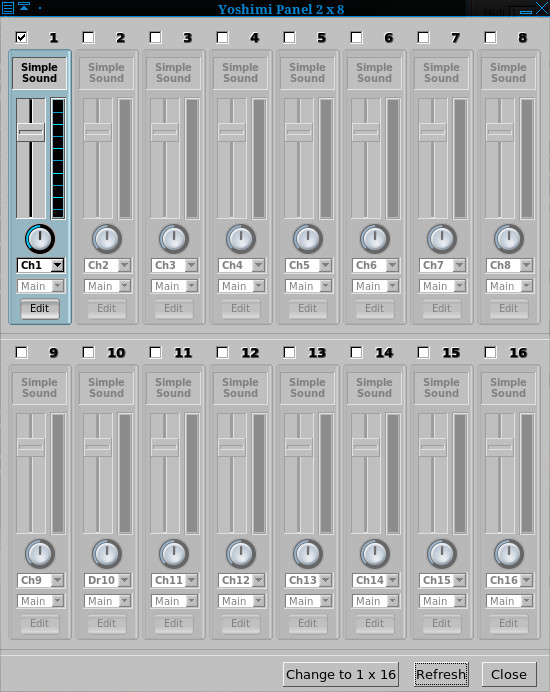
\includegraphics[scale=1.0]{top-panel/yoshimi-panel-2x8.jpg}
   \caption[Yoshimi Part Panel]{Yoshimi Part Panel, 2x8}
   \label{fig:yoshimi_part_panel_2x8}
\end{figure}

   \setcounter{ItemCounter}{0}      % Reset the ItemCounter for this list.

   \itempar{Part Summary}{Part Section, 1 to 16}
   Parts View or Summary.

   \itempar{Enable part}{parts!enable}
   Enable/Disable the part. The check-box enables/disables the part.
   When the part is disabled, its controls are greyed out.

   Values: \texttt{Off*, On}

   \itempar{Part name}{parts!name}
   Instrument name. Click on this box to change the instrument (it will
   open up the \textbf{Edit} window.

   \itempar{Volume Slider}{parts!volume}
   Volume Bar.
   Changes the volume of the part.

   \itempar{VU-meter display}{parts!meter}
   Shows the level of the part when playing.

   \itempar{Panning Knob}{parts!panning}
   Panning Dial-Button.
   Changes the panning of the part.

   \itempar{Channel}{parts!channel}
   Receive from MIDI channel.
   Changes the MIDI channel assigned to the part.

   Values: \texttt{Ch1*, Ch2, ..., Ch16}

   \itempar{Main}{parts!destination}
   Set Audio Destination.
   Sets the audio for this part to be routed to the main audio output, to
   the audio specified by the part setup, or to both outputs.
   This option requires that \textsl{Yoshimi} use JACK audio.  If running
   ALSA, this option is disabled (greyed out).

   Values: \texttt{Main, Part, or Both}

   The part audio destination (JACK) is saved with the parameter sets, and
   so is the number of available parts.  (\textsl{ZynAddSubFX} will still
   load these files, but it ignores any settings it doesn't recognise. If
   one re-saves in \textsl{ZynAddSubFX}, the settings will be lost.)

   \itempar{Edit}{parts!edit}
   The Edit button provides two function
   Left mouse button: Part select.
   Right mouse button: Instrument edit.

   \textsl{This is a bit unintuitive.  The left/right clicks could be
   reversed, and the button named something like "Edit/Pick".}

   \itempar{Parts Layout}{parts!change layout}
   \index{parts!2x8}
   \index{parts!1x16}
   Changes the layout of the panel.

   \itempar{Refresh}{obsolete!refresh}
   Refresh Edit. OBSOLETE.

   \itempar{Close}{parts!close}
   Close the window.

\subsection{Virtual Keyboard}
\label{subsec:virtual_keyboard}

   This section describes the detailed usage of the
   \textsl{Yoshimi} virtual keyboard.
   The virtual keyboard lets one play notes using the keyboard/mouse. There is
   no MIDI requirement. 
    
   Using the keyboard. The keyboard is split into two "octaves"(in fact it is
   more than 1 octave). It may happen that the keys will not trigger any
   note-on This is because another widget than the keyboard itself is selected.
   In order to continue playing using the keyboard, click with the mouse on
   some keys on the virtual keyboard.
   
   Using the mouse. One can use the mouse too, to play.
   If one presses the shift key while pressing the mouse button,
   the keys will be not released when the mouse button is released.  If one
   presses the "Panic" or "Stop!" button from the ZynAddSubFX/Yoshimi
   main window, all keys will be released. 

\begin{figure}[H]
   \centering 
   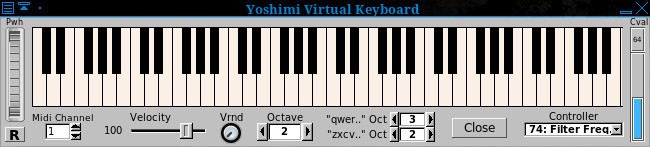
\includegraphics[scale=1.0]{top-panel/yoshimi-virtual-keyboard.jpg}
   \caption{Yoshimi Virtual Keyboard}
   \label{fig:yoshimi_virtual_keyboard}
\end{figure}

\subsubsection{Virtual Keyboard, Basics}
\label{subsubsec:virtual_keyboard_basics}

   \begin{enumber}
      \item \textbf{Pwh}
      \item \textbf{R}
      \item \textbf{Midi Channel}
      \item \textbf{Velocity}
      \item \textbf{Velocity}
      \item \textbf{Octave}
      \item \textbf{"qwer.." Oct}
      \item \textbf{"zxcv.." Oct}
      \item \textbf{Controller}
      \item \textbf{Cval}
      \item \textbf{Close}
   \end{enumber}

   \itempar{Pwh}{vkdb!pitch bend}
   Pitch bend knob. Pitch wheel.
   Press the \textbf{R} button to reset it.

   \itempar{R}{vkdb!reset pitch bend}
   Reset Pitch Bend.

   \itempar{Midi Channel}{vkdb!midi channel}
   MIDI Channel.
   Sets the MIDI channel for the virtual keyboard.

   Values: \texttt{1* to 16}

   \itempar{Velocity}{vkdb!velocity}
   Velocity of Notes.
   Sets the note-on velocity for the virtual keyboard.

   Values: \texttt{1 to 127, 100*}

   \itempar{Velocity}{vkdb!velocity randomness}
   Velocity Randomness.

   Values: \texttt{0* to 127}

   \itempar{Octave}{vkdb!qwerty}
   Transposes all of the virtual keyboard notes by the given number of
   octaves.

   Values: \texttt{1, 2*, 3, 4, 5}

   \itempar{"qwer.." Oct}{vkdb!qwert}
   q2w3e4r5t6y Octave.
   Transposes the upper keys ("qwert"); the range of these keys is from C-4
   to A-5 (replace the '5' with the octave).

   \itempar{"qwer.." Oct}{vkdb!zxcvb}
   zsxdcfvgbh Octave.
   Transposes the lower keys ("zxcvb"); the range of these keys is from C-3
   to E-4 (replace the '4' with the octave).

   Values: \texttt{1, 2*, 3, 4, 5}

   \itempar{Controller}{vkdb!controller}
   Keyboard Controller.

   Values: \texttt{01:Mod.Wheel, 07:Volume, 10:Panning,
      11:Expression, 64:Sustain, 65:Portamento, 71:Filter Q,
      74:Filter Freq*, 75:Bandwidth, 76:FM Gain,
      77:Res.c.freq, 78:Res.bw.}

   Sets the controller to be changed according to Cval.
   See \sectionref{subsubsec:virtual_keyboard_controllers}.

   \itempar{Cval}{vkdb!controller value}
   Controller value.
   Changes the controller value. Note that the Cval might not reflect the
   internal value of the controller when one changes the controller.

   Values: \texttt{1 to 127, 96*}

   \itempar{Close}{vkdb!close}
   Close button.

\subsubsection{Virtual Keyboard, ASCII Mapping}
\label{subsubsec:virtual_keyboard_ascii}

   In addition to this virtual keyboard, the QWERTY (or Dvorak, or AZERTY)
   keyboards can be used to produce notes.
   The computer keyboard layout is shown in
   \figureref{fig:qwerty_virtual_keyboard},
   From lowest octave to highest, the colors are blue, then green, then red.
   The "white" keys are the light colors, and the "black" keys are the
   deeper colors.
   The range of the keys on the "zxcvb..." row is C3 to E4.
   The range of the keys on the "qwert..." row is C4 to A5.
   These octave ranges can be adjusted.

   The computer keyboard will produce notes only when the virtual keyboard
   is active.

   TODO: Note that there may be some other keys that serve a purpose with
   the QWERTY keyboard.

   Also note that we replaced the monopoly symbol with the monopolist
   symbol.  On X11 systems, this key is known as the "Super" key.

\subsubsection{Virtual Keyboard, Controllers}
\label{subsubsec:virtual_keyboard_controllers}

   \begin{enumber}
      \item \textbf{Mod. Wheel}
      \item \textbf{Volume}
      \item \textbf{Panning}
      \item \textbf{Expression}
      \item \textbf{Sustain}
      \item \textbf{Portamento}
      \item \textbf{Filter Q}
      \item \textbf{Filter Freq.}
      \item \textbf{Bandwidth}
      \item \textbf{FM Gain}
      \item \textbf{Res. c. freq}
      \item \textbf{Res. bw.}
   \end{enumber}

% The following diagram is actually in the the wrong directory, it is really
% a top-panel diagram.

\begin{figure}[H]
   \centering 
   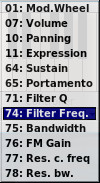
\includegraphics[scale=0.5]{menu/Instrument/virtual-keyboard-controllers.jpg}
   \caption{Virtual Keyboard Controllers}
   \label{fig:virtual_keyboard_controllers}
\end{figure}

   \setcounter{ItemCounter}{0}      % Reset the ItemCounter for this list.

   \itempar{Mod. Wheel}{controllers!modulation wheel}

   TODO.

   \itempar{Volume}{controllers!volume}

   TODO.

   \itempar{Panning}{controllers!panning}

   TODO.

   \itempar{Expression}{controllers!expression}

   TODO.

   \itempar{Sustain}{controllers!sustain}

   TODO.

   \itempar{Portamento}{controllers!portamento}

   TODO.

   \itempar{Filter Q}{controllers!filter q}

   TODO.

   \itempar{Filter Freq.}{controllers!filter frequency}

   TODO.

   \itempar{Bandwidth}{controllers!bandwidth}

   TODO.

   \itempar{FM Gain}{controllers!fm gain}

   TODO.

   \itempar{Res. c. freq}{controllers!resonant center frequency}

   TODO.

   \itempar{Res. bw.}{controllers!resonant bandwidth}

   TODO.

%-------------------------------------------------------------------------------
% vim: ts=3 sw=3 et ft=tex
%-------------------------------------------------------------------------------
